\documentclass{beamer}
\usetheme {CambridgeUS}
\usepackage{listings}
\usepackage{upquote}
%\setbeameroption{hide notes} % Only slides
%\setbeameroption{show only notes} % Only notes
\setbeameroption{show notes on second screen=right} % Both

\title{Docker deep dive}
\subtitle{How we leverage the Docker stack}
\author[Ezri Zhu]{Ezri Zhu \\ tzhu22@stevens.edu \\ \url{https://ezrizhu.com}}
\institute[Blueprint@Stevens]{Bluepring @ Stevens Institute of Technology}
\date{\today}

\begin{document}

\begin{frame}
    \titlepage


    \note[item]{Hello, my name is Ezri Zhu I am a second year computer science undergrad at the Stevens Institute of Technology}
    \note[item]{I have been the VP of tech at blueprint since last year. There
    will be a Q\&A at the end, tho feel free to interrupt me during the
    presentation for questions.}
\end{frame}

\begin{frame}
    \includegraphics[scale=0.10]{img/DockerLogo}\\
    \vspace{5mm}
    \begin{itemize}
    \item Dockerfile, Docker Images \\
    \item Docker Container \\
    \item Docker Registry \\
    \item Docker-compose \\
    \end{itemize}

    Logo credit: https://github.com/Aikoyori/ProgrammingVTuberLogos/
    \note[item]{In this talk I will do a overview of the different components of
    a typical docker deployment, then we'll get into how exactly we're
    leveraging Docker at Blueprint}
\end{frame}

\begin{frame}{What's Docker for? - The Bigger Picture}

    Docker simplifies software development and deployment by packaging
    applications and their dependencies into portable containers, that their
    behavior are the same across different environment.

    \begin{itemize}
        \item Developer develops their application
        \item Developer writes a Dockerfile, defining how to package their
            application in a docker container
        \item Developer builds the Dockerfile into an image, pushes to a registry
        \item Developer pulls the image from the registry on the deployment
            server
        \item At the same time, developer 2 can also pull the same image and
            test it on their machine
    \end{itemize}

    \note[item]{I will first give you a quick overview of how docker is used in
    a typical development cycle}
    \note[item]{We're mostly software developers here, and I am sure most of you
    have ran into the issue where someone's application doesn't work on someone
    elses computer}
    \note[item]{Those issues are usually solved by dependency issues, a certain
    python application may rely on a bunch of other python dependencies, and
    your systems package manager may also provide these packages but under
    different versions, thus also breaking seeemly working deployments}
    \note[item]{With docker, you define exactly what the environment is, from
    the base OS image that the container is built from, to unpacking your
    application}
\end{frame}

\begin{frame}{Linux Namespace via unshare}
    This is your computer, a program usually have access to all of these system resources provided by the Kernel. \\
    By default, processes you call will inherit all of your namespaces\\
    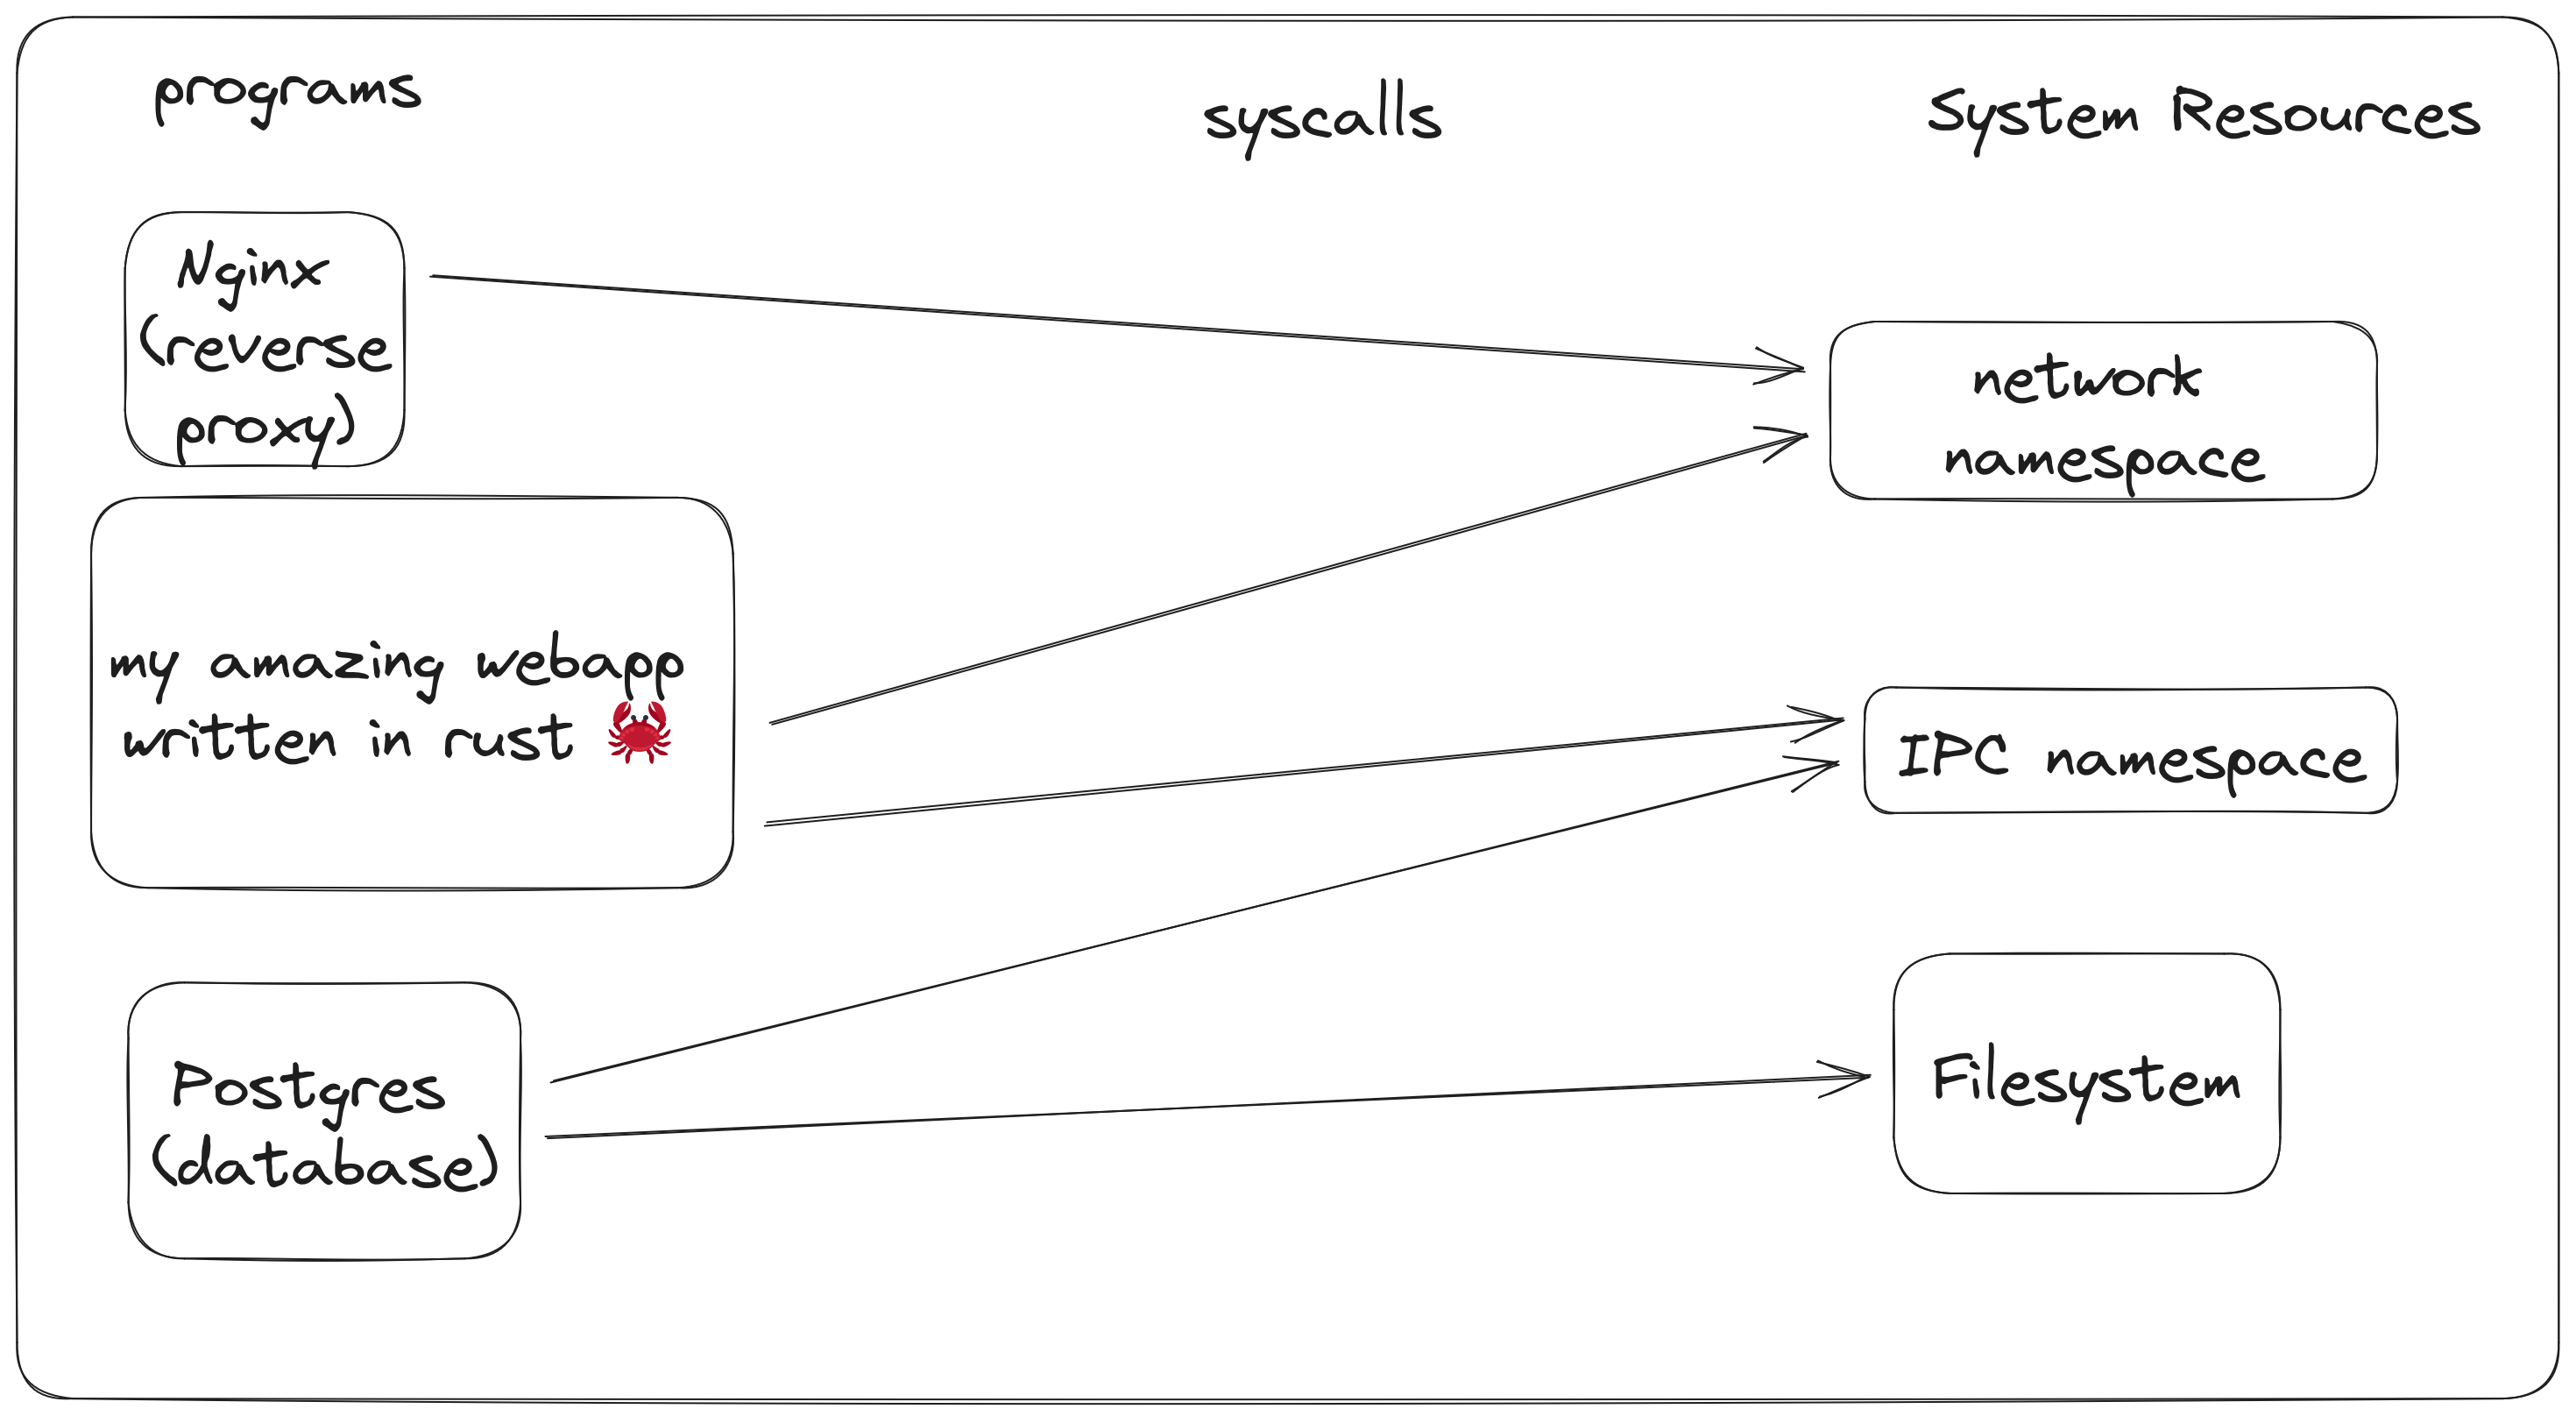
\includegraphics[scale=0.10]{img/unshare-1}\\
    \note[item]{This is your computer, a program usually have access to all of these system resources provided by the Kernel.}
    \note[item]{By default, processes you call will inherit all of your namespaces, just like how when you prefix a command with sudo, it will inherit all of root's permissions}
    \note[item]{Here, you will notice three programs, a nginx reverse proxy, a postgres database, and my amazing webapp written in rust}
    \note[item]{As you can see, nginx is able to reverse proxy the webapp because they both share a network namespace}
    \note[item]{Then, the webapp is able to communicate with the postgres database via a socket, so that's done in the IPC namespace}
    \note[item]{There are other namespaces (PID, filesystem mounts, control groups, users), but we will pretend they don't exist for now for the sake of simplicity.}
\end{frame}

\begin{frame}{Linux Namespace via unshare}
    TD's Computer (he's a bit paranoid)\\
    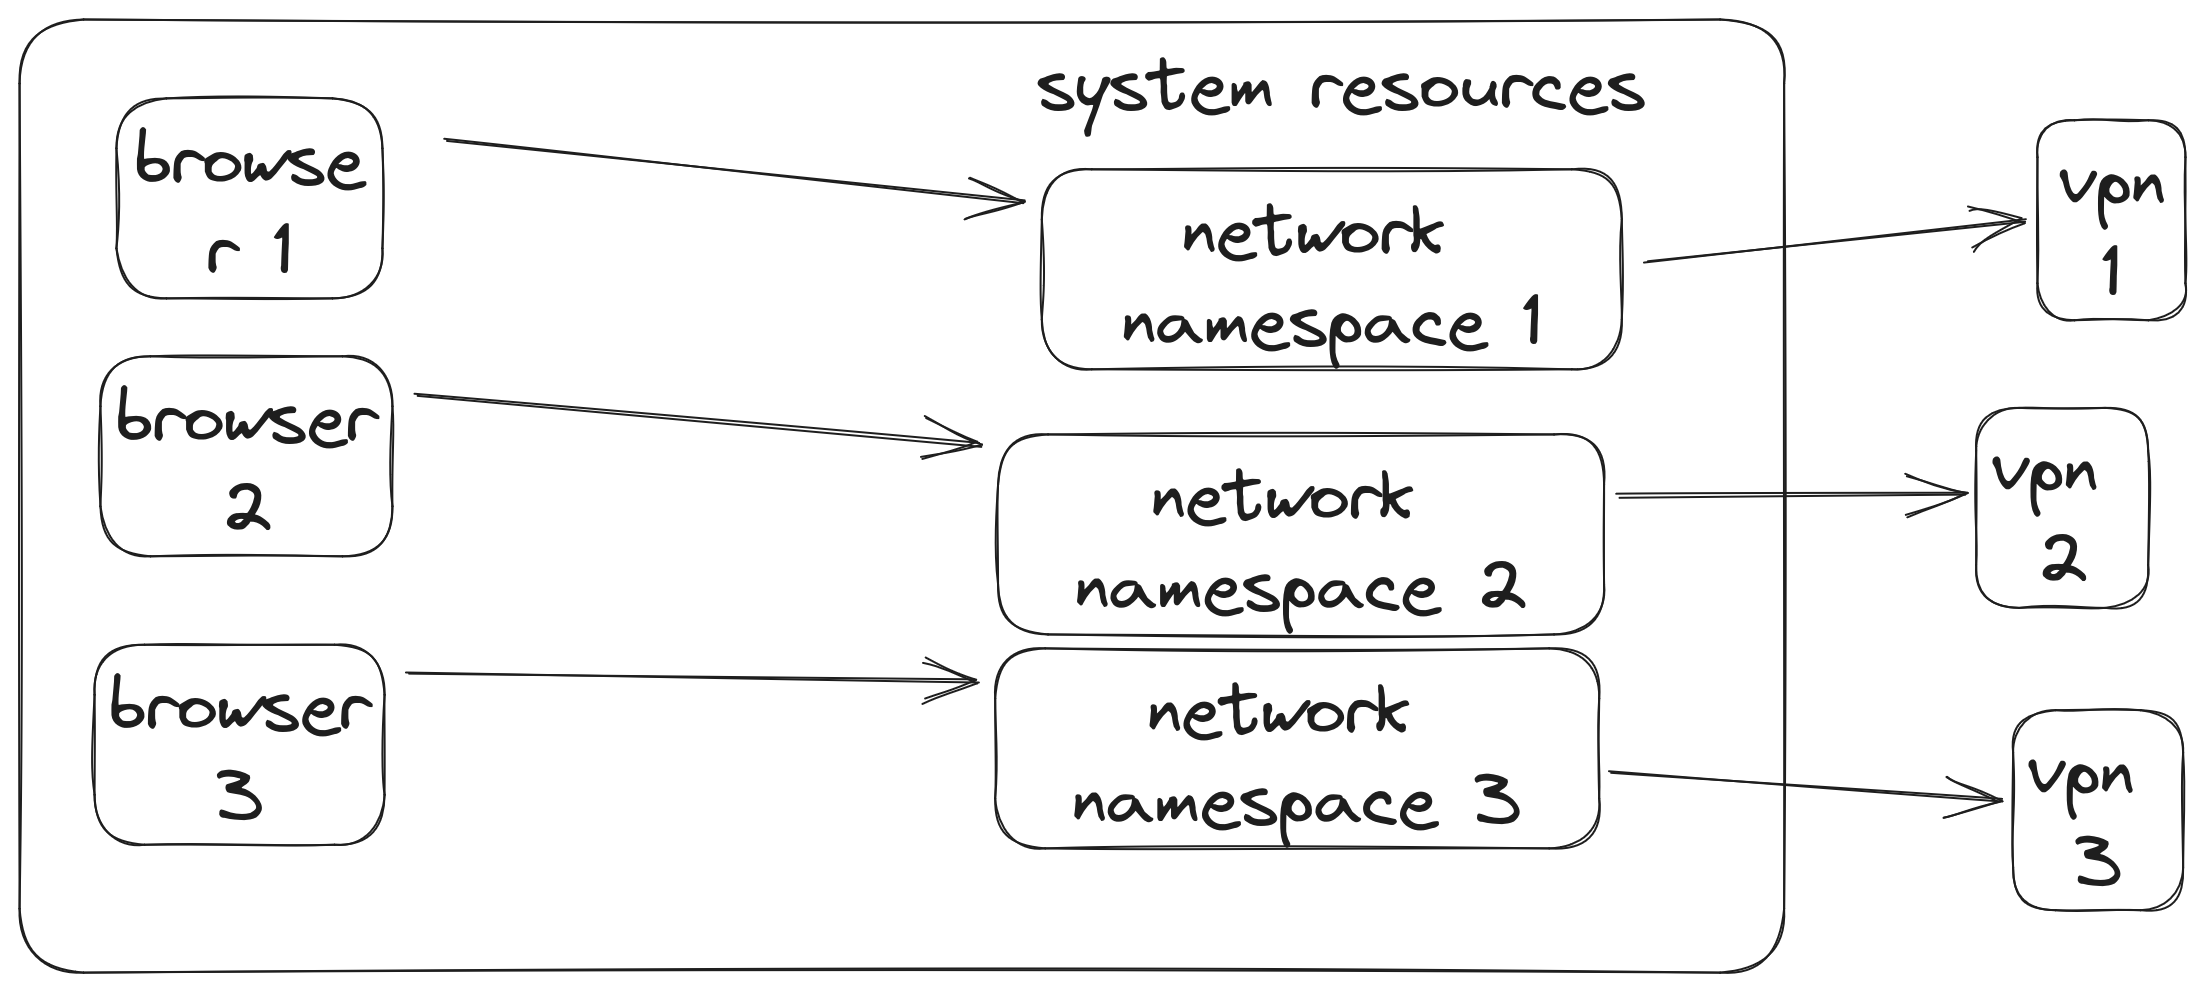
\includegraphics[scale=0.10]{img/unshare-2}

    \note[item]{Here is an example of linux namespaces being used in the real world}
    \note[item]{TD has a computer and he really doesn't want to be tracked by ad companies and other organizations on the internet.}
    \note[item]{So he has three VPN setup in three separate linux network namespaces.}
    \note[item]{He then spawns a browser in each of the three namespaces, where he will work on different things.}
    \note[item]{This allows him to have three different IP addresses on the browser.}
\end{frame}

\begin{frame}{Overlayfs}
    How overlayfs works\\
    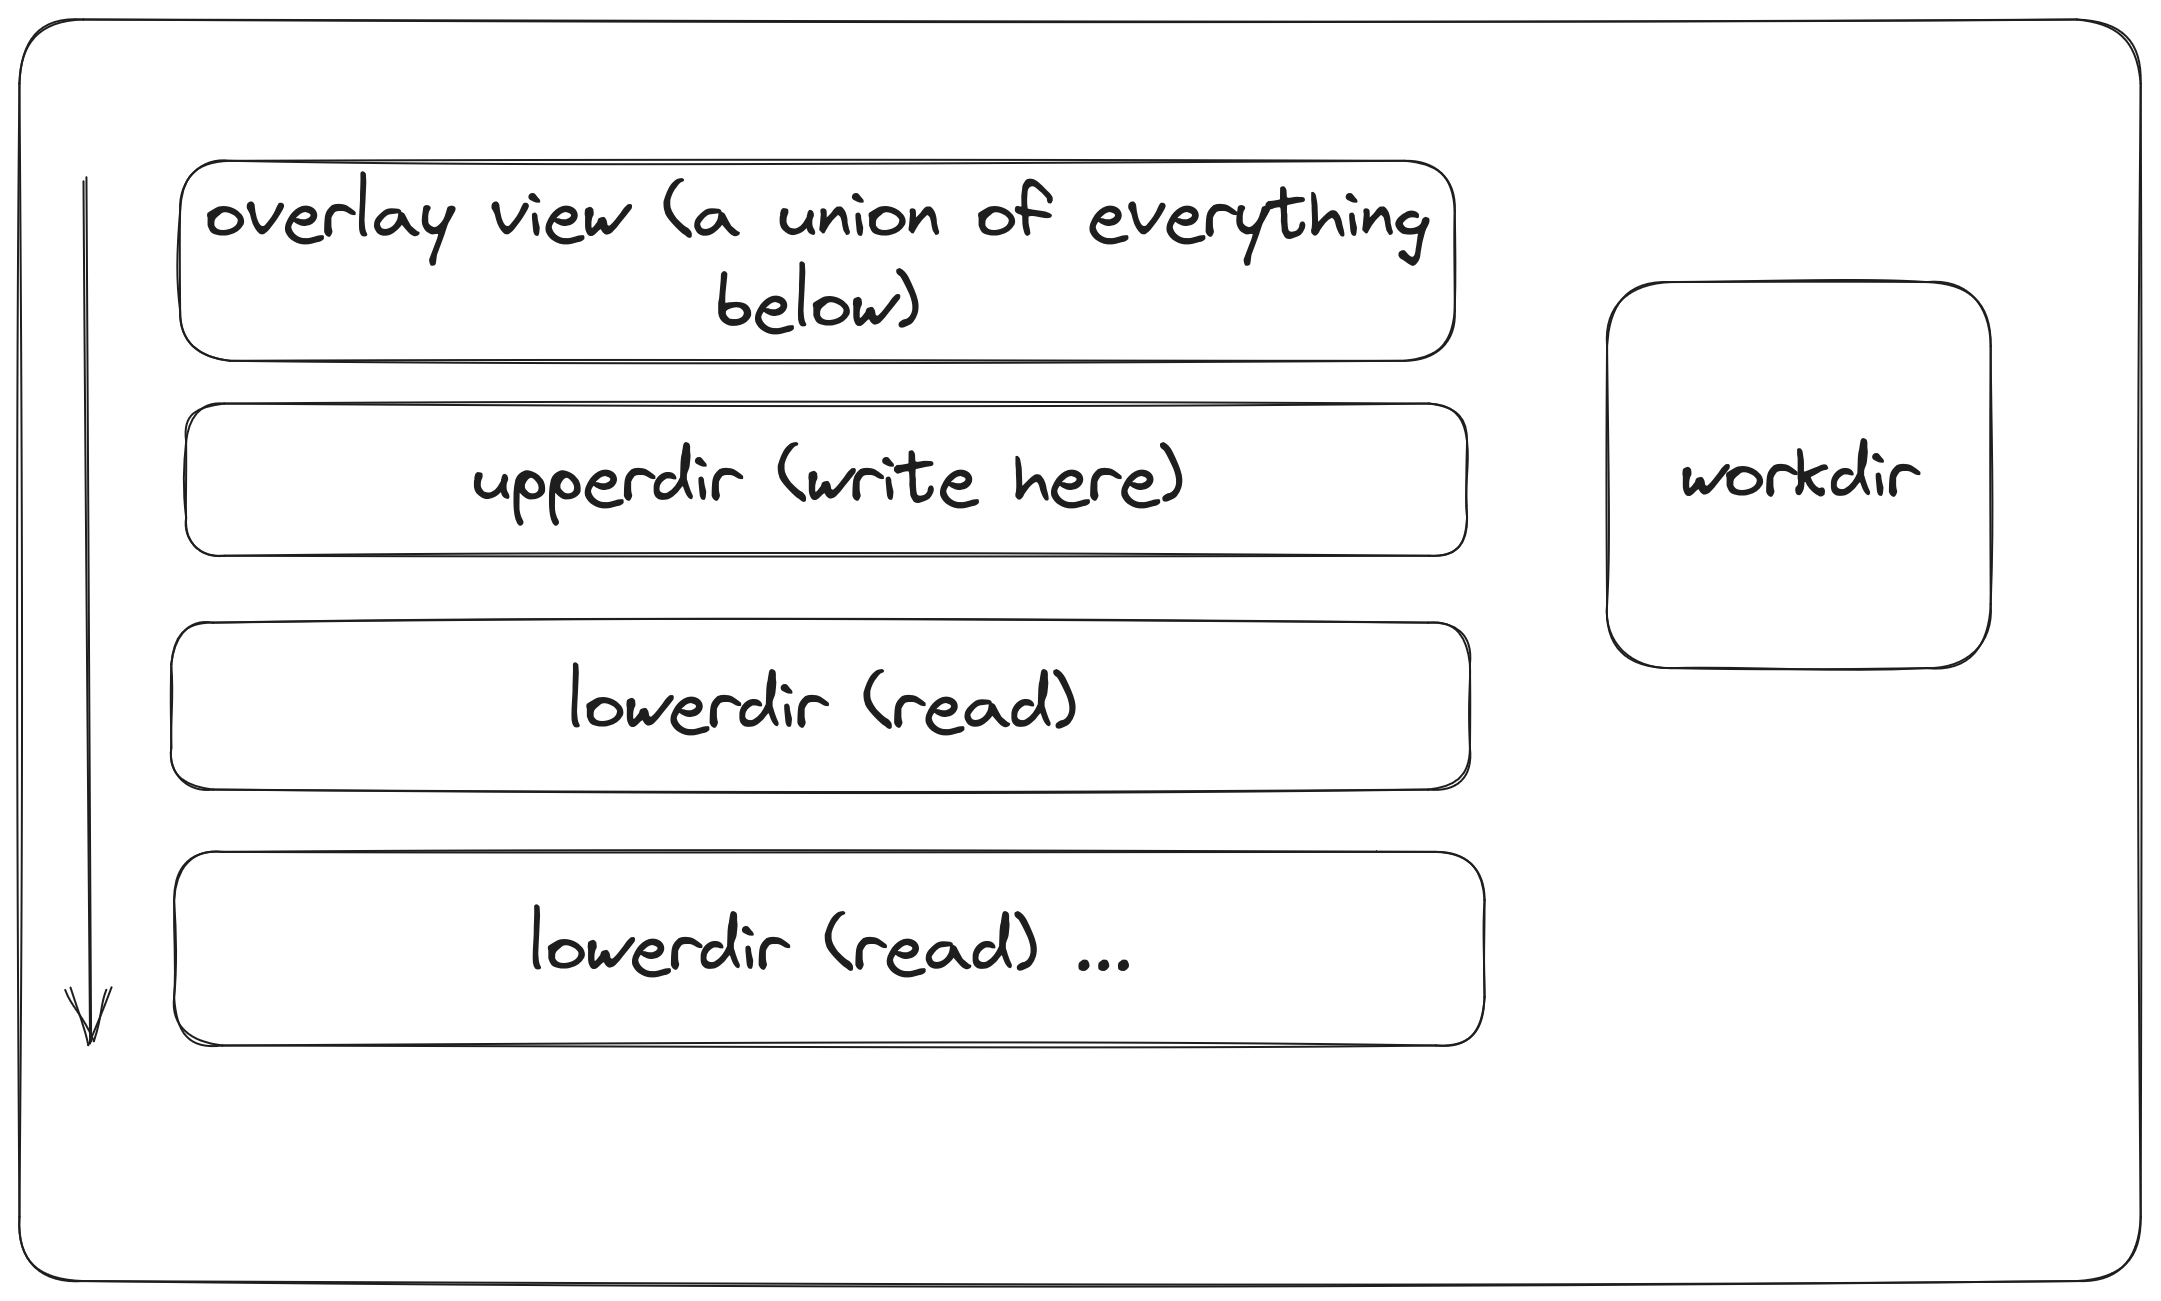
\includegraphics[scale=0.10]{img/overlayfs-1}\\
    \url{https://docs.kernel.org/filesystems/overlayfs.html}

    \note[item]{Overlayfs at minimum uses four directories, a lowerdir, a upperdir, a workdir, and a directry to mount the merged view of everything}
    \note[item]{lowerdir contains everything that were already in the system, and overlayfs will not write to it}
    \note[item]{the merged directory, which we labled as overlay view on the diagram, is where we will be interacting with overlayfs}
    \note[item]{upperdir is where overlayfs will write changes to when they are made in the merged directory.}
    \note[item]{workdir is where overlay stage changes to as it is copying files up from lowerdir to upperdir}
\end{frame}

\begin{frame}{Overlayfs}
    Beginning state\\
    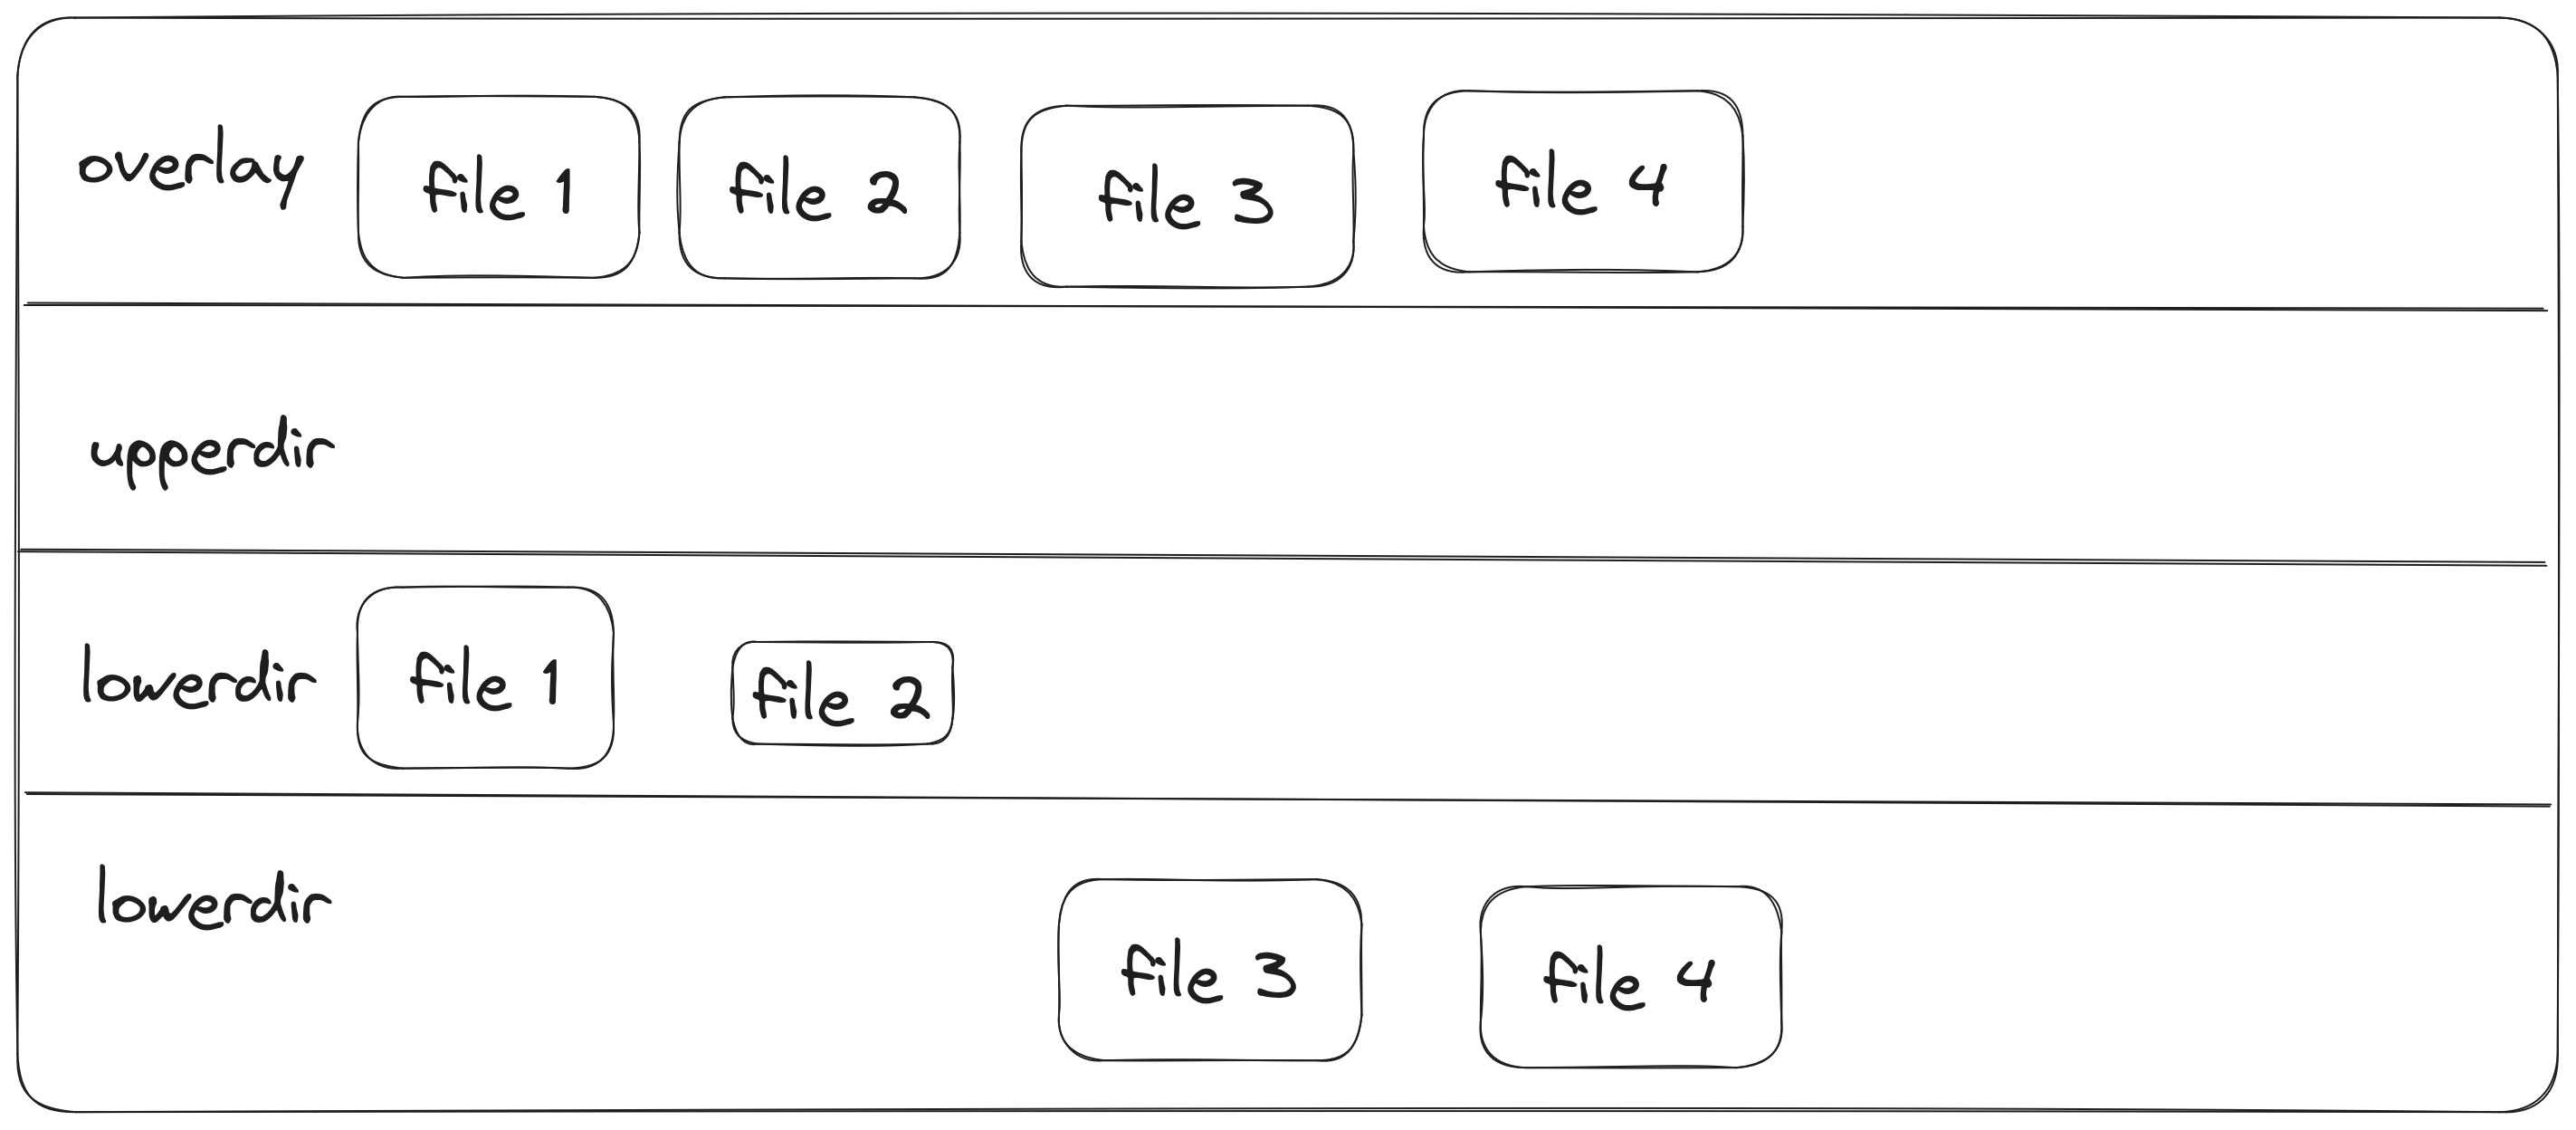
\includegraphics[scale=0.10]{img/overlayfs-2}

    \note[item]{For example, we have two directories, lowerdir 1, and lowerdir 2, and they each contains two files}
    \note[item]{You don't need to have two lower-directories, and when you first start overlayfs with two lowerdirs, it will just merge the two}
    \note[item]{You will have to give overlayfs three empty directories, one for the upperdir, one for the workdir, and one to mount the overlay view to}
    \note[item]{after overlayfs is mounted to the overlay view, you are able to see the four files from the two lower directories in from the overlay view}
\end{frame}

\begin{frame}{Overlayfs}
    Makes file 5, edits file 1\\
    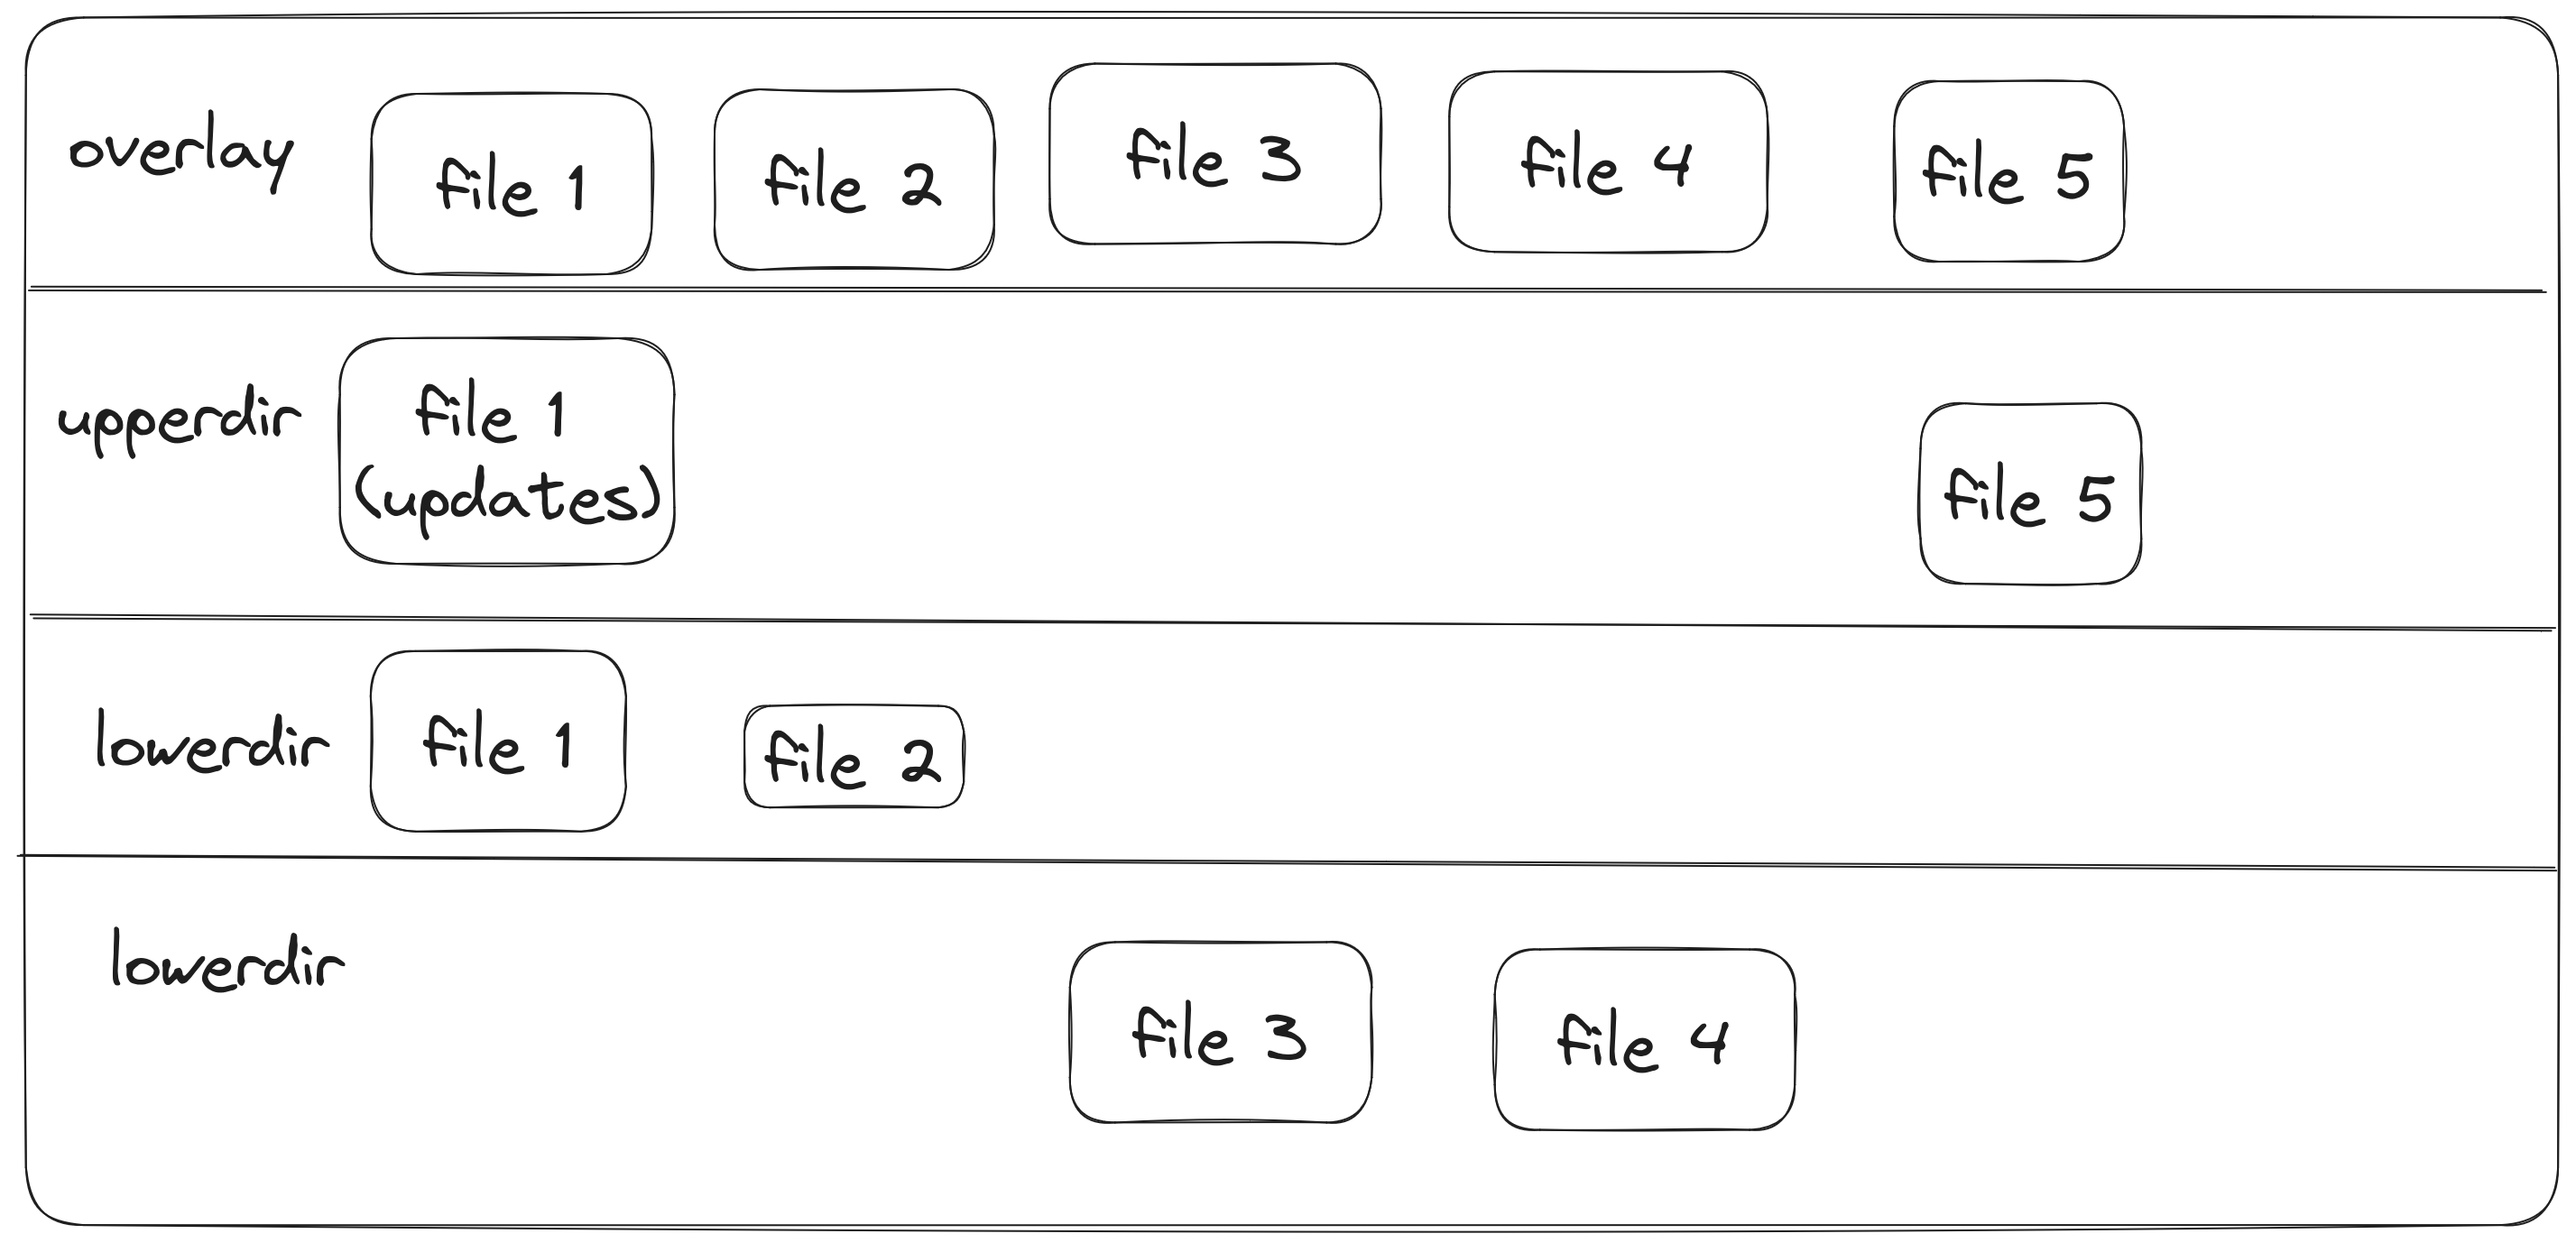
\includegraphics[scale=0.10]{img/overlayfs-3}

    \note[item]{Here we'll make a new file called file 5, and we will edit file 1}
    \note[item]{As you can see, overlayfs writes the updated file 1, and creates file 5 in upperdir, leaving lowerdir alone. However, the changes are reflected in the overlay view}
\end{frame}

\begin{frame}{Overlayfs}
    Deletes file 2\\
    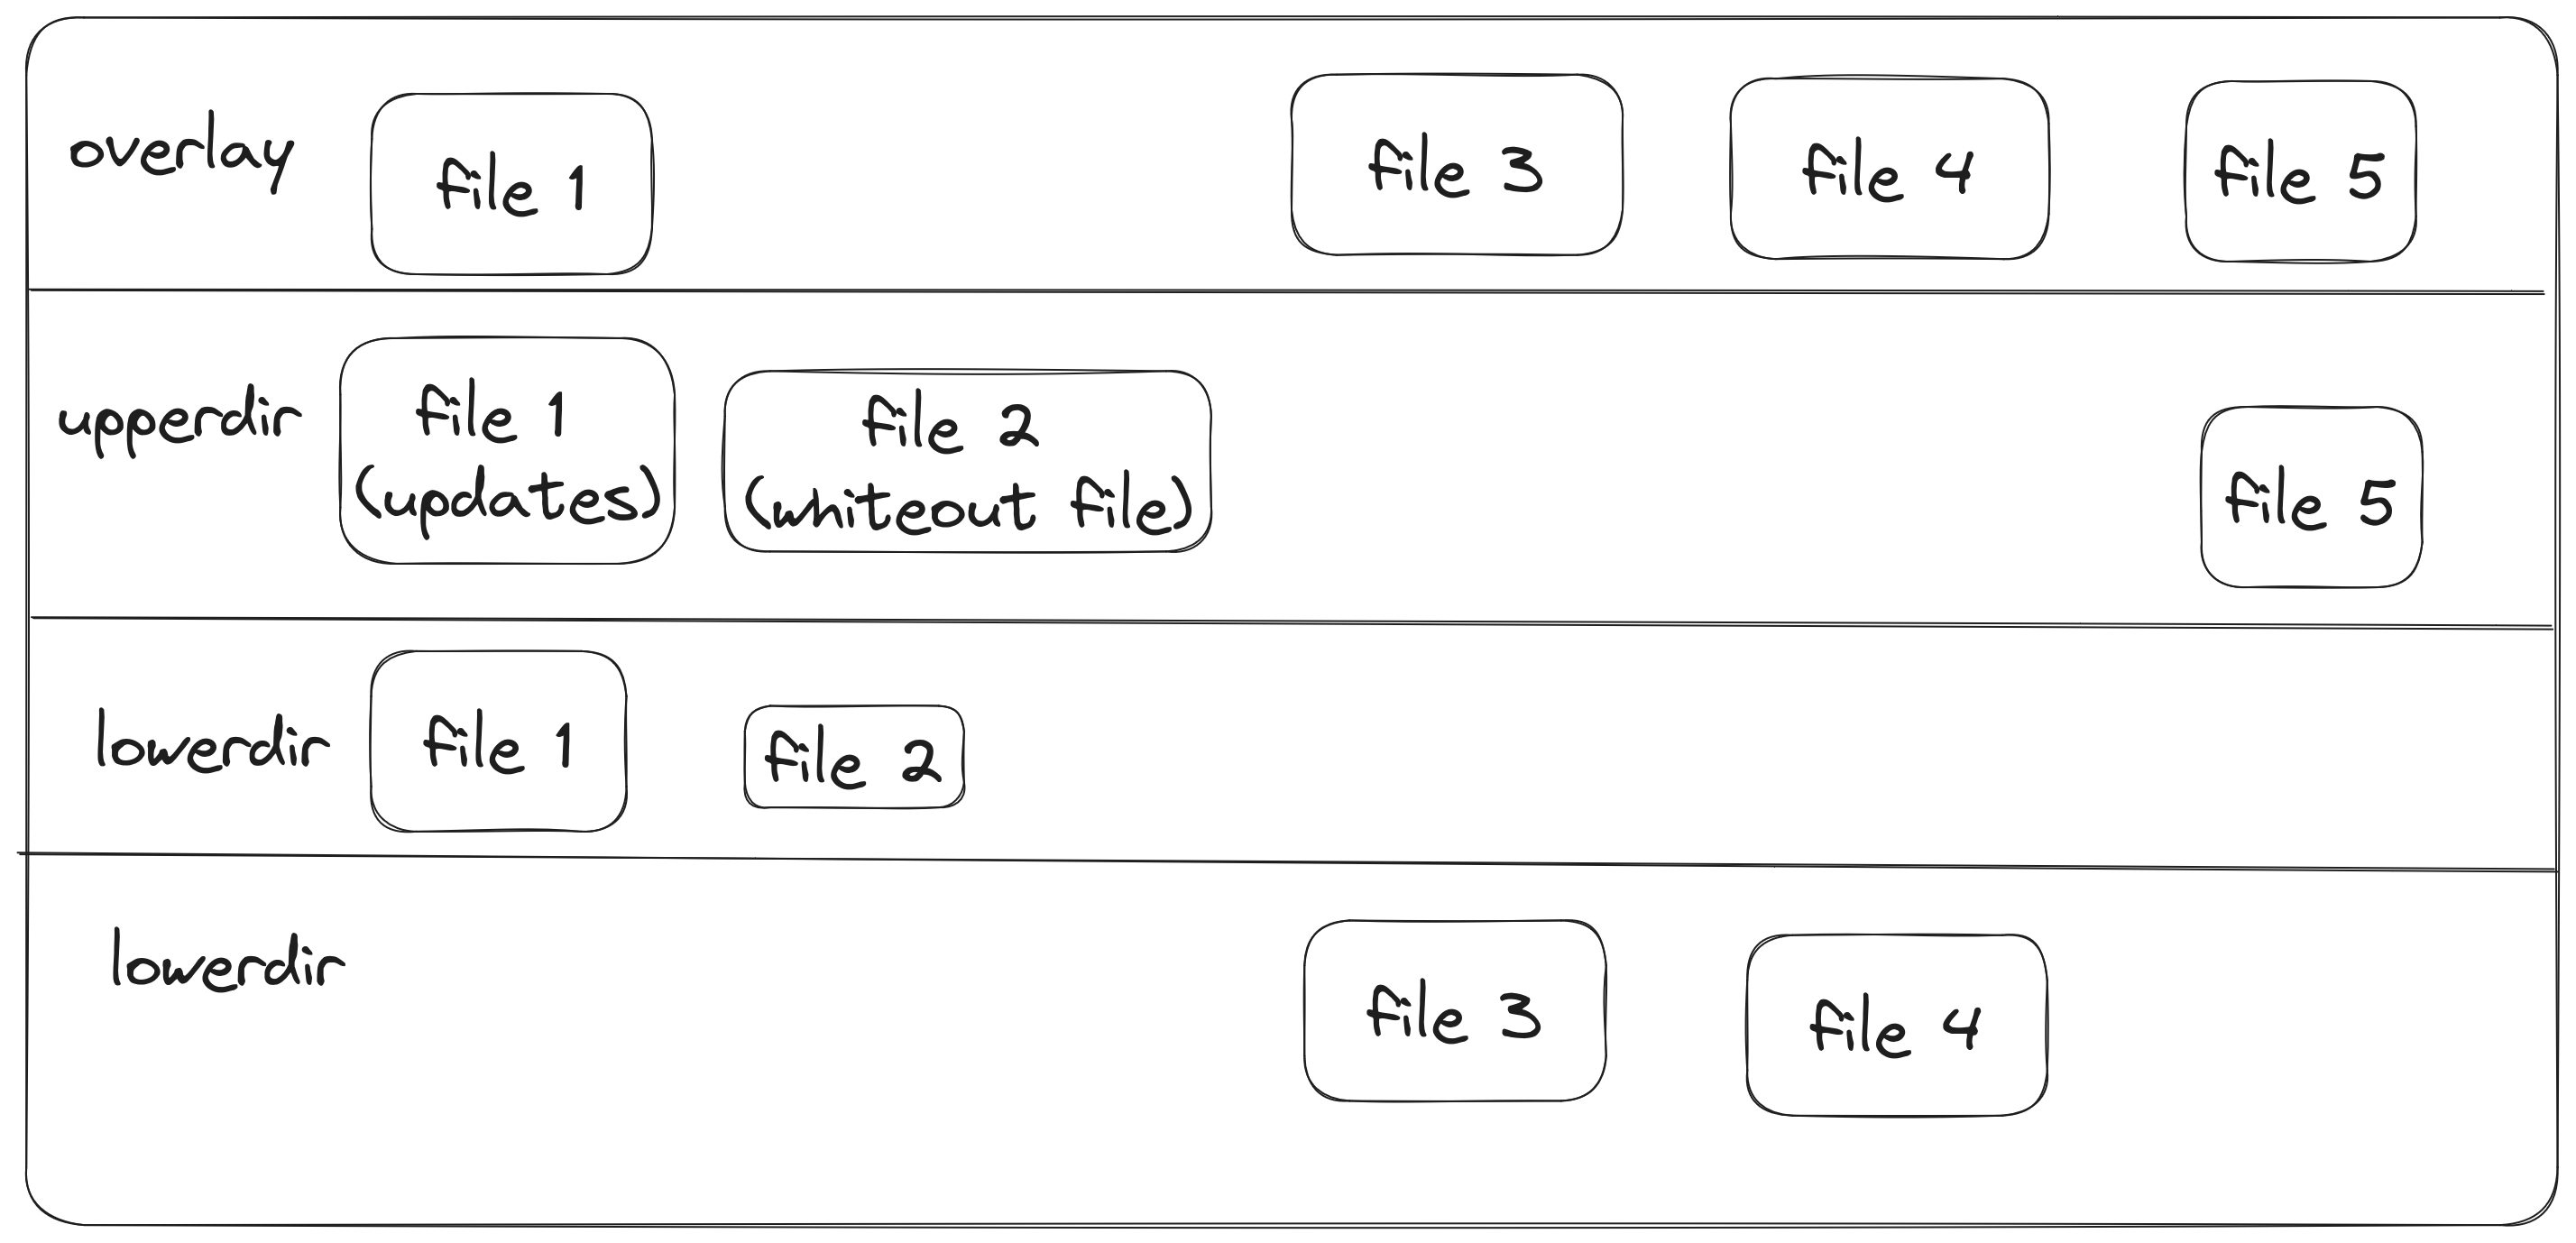
\includegraphics[scale=0.10]{img/overlayfs-4}

    \note[item]{Here, we will delete file two. For file deletions, overlayfs will write a character device at the location of the file that it is removing, and the file will disappear from the overlay view}
    \note[item]{You probably didn't understand all of that, but the main
    takeaway is that overlayfs allows us to stack filesystems on top of each
    other like a hamburger, and if we want to add some files, we just add a
    lettuce on the top with more files, if we want to remove some files, we
    add a lettuce on the top with a hole at where the file is}
    \note[item]{And that's how docker images are built, its just a big hamburger
    of layers of filesystem states}
\end{frame}

\begin{frame}[fragile]{Overlayfs}
    \tiny
    \begin{lstlisting}
mount -t overlay overlay \
-o "lowerdir=$lowerdir1,$lowerdir2,upperdir=$upperdir,workdir=$workdir" "$overlay"
    \end{lstlisting}
    \normalsize
    \note{And this is how you start an overlay mount}
\end{frame}

\begin{frame}[fragile]{Overlayfs}
    \tiny
    \begin{lstlisting}
$ docker pull postgres
Using default tag: latest
latest: Pulling from library/postgres
a803e7c4b030: Pull complete
009c876521a0: Pull complete
9c412905cca2: Pull complete
6463d4bf467a: Pull complete
bd8b983728ed: Pull complete
febc167f3560: Pull complete
d73c81c4ade3: Pull complete
34b3b0ac6e9e: Pull complete
9bd86d074f4e: Pull complete
406f63329750: Pull complete
ec40772694b7: Pull complete
7d3dfa1637e9: Pull complete
e217ca41159f: Pull complete
Digest: sha256:f1aaf6f8be5552bef66c5580efbd2942c37d7277cd0416ef4939fa34bf0baf31
Status: Downloaded newer image for postgres:latest
docker.io/library/postgres:latest
    \end{lstlisting}
    \normalsize

    \note[item]{And this is also how docker works, when you build a container, each line in the dockerfile is being written to it's own upperdir, with everything preceding are just lowerdirs in a merged view}
    \note[item]{So when you pull a docker image and run it, each layer is just a lowerdir, and your container is mounted on the overlay view}
\end{frame}

\begin{frame}[fragile]{Dockerfile}
    A Quick Example\\

    \begin{lstlisting}
FROM node:20
WORKDIR /app 
COPY . .
RUN npm i
RUN npm run build
EXPOSE 3000
CMD ["npm", "run", "start"]
    \end{lstlisting}

    \note[item]{This is a pretty standard Dockerfile for a node application,
    packed by npm}
    \note[item]{First, we pull the node:20 image, maintianed by the nice people
    over at nodejs, this allows us to pin our node version to be at 20}
    \note[item]{Second, we set the working directory to /app, this is the same
    as doing cd in the container}
\end{frame}

\begin{frame}[fragile]{Building a docker image}

    docker build -t ghcr.io/stevensblueprint/project:ezri-latest .

    \note[item]{In the same directory as the Dockerfile, we can now build the
    docker image}
    \note[item]{Docker images are named via labels, a image can have mutlple
    labels}
    \note[item]{Each image has a hash, it's basically the image's unique ID}
    \note[item]{But we can also give it a more human readable name, consisted of
    a path and a tag}
    \note[item]{usually a path denotes what the application is, such as the name
    of the repository}
    \note[item]{and a tag denotes the version that the application is}
\end{frame}

\begin{frame}[fragile]{Building a docker image}

    docker build -t app . \\
    docker tag app ghcr.io/stevensblueprint/project:ezri-latest \\
    docker tag app ghcr.io/stevensblueprint/project:latest \\
    docker tag app ghcr.io/stevensblueprint/project:staging \\

    \note[item]{In the same directory as the Dockerfile, we can now build the
    docker image}
    \note[item]{Docker images are named via labels, a image can have mutlple
    labels}
    \note[item]{Each image has a hash, it's basically the image's unique ID}
    \note[item]{But we can also give it a more human readable name, consisted of
    a path and a tag}
    \note[item]{usually a path denotes what the application is, such as the name
    of the repository}
    \note[item]{and a tag denotes the version that the application is}
\end{frame}

\begin{frame}[fragile]{Pushing a docker image}

    docker push ghcr.io/stevensblueprint/project:ezri-latest \\
    docker push ghcr.io/stevensblueprint/project:latest \\
    docker push ghcr.io/stevensblueprint/project:staging \\

    \note[item]{Now, we can use docker push to push it to the docker registery}
    \note[item]{In our case, we're using ghcr.io, which is the github container
    registry}
    \note[item]{That's basically a place where we store our container images,
    and we can pull them from other places}
\end{frame}

\begin{frame}[fragile]{Launching a docker container}

docker run --name app-test -p 8080:8080
    ghcr.io/stevensblueprint/project:ezri-latest \\
    
    Full options here:
    https://docs.docker.com/reference/cli/docker/container/run/ \\
\end{frame}

\begin{frame}[fragile]{Writing a docker compose file}

    \begin{lstlisting}
services:
  redis:
    image: redis:latest
    restart: always
    ports:
      - "6379:6379"
  api:
    build:
      dockerfile: Dockerfile
      context: .
    restart: always
    ports:
      - "8080:8080"
    depends_on:
      - redis

volumes:
  redis:
    driver: local
    \end{lstlisting}
    
\end{frame}

\begin{frame}[fragile]{Launching a docker compose}

docker compose up (-d) \\
docker compose down \\
docker compose ps \\
docker compose logs \\

\end{frame}

\begin{frame}{Recap}
    Dockerfile: Defines a docker image\\
    Docker Image: A portable runtime environment\\
    Docker registry: A place to store docker images\\
    Docker container: A running instance of a docker image\\
    Docker compose: A collection of docker containers and its dependencies\\
\end{frame}

\begin{frame}{nuances missed}
    OCI Containers vs Docker contianers \\
    Look into: github.com/containers/crun \\
    Also see also: mobyproject.org/ \\

    \note[item]{docker is not the only way to do linux contianers, but for the
    sake of simplicity this ppt only talked ab dockers}
    \note[item]{Feel free to also ask about how we're using github actions to
    build and test, and deploy docker containers in our CI/CD workflow}
\end{frame}

\begin{frame}{related tech}
    firecracker MVM (orig): firecracker-microvm.github.io
    firecracker MVM (flyio): fly.io/blog/sandboxing-and-workload-isolation\\
    v8 isolates (cf talk) www.infoq.com/presentations/cloudflare-v8 \\
    v8 isolates (cf security)
    developers.cloudflare.com/workers/reference/security-model \\
    v8 isolates (deno edition) deno.com/blog/anatomy-isolate-cloud \\
    v8 isolates (deno but diff) blog.val.town/blog/first-four-val-town-runtimes \\
    Nix, Flakes, NixOS \\

    \note[item]{basically other ways we run/scale applications}
    \note[item]{happy to talk ab them after the talk}
\end{frame}

\begin{frame}{Thank you!}
    Questions? \\
\end{frame}

\end{document}
